\subsection{Virtualisation Techniques}

Traditionally virtualisation has referred to a software abstraction layer residing between the computer hardware and the operating system. \cite{taxonomy} This layer has been called Virtual Machine Monitor (VMM) or more recently a hypervisor and it hides and abstracts the computing resources from the OS, allowing multiple OSs to run simultaneously on the same hardware. There are multiple ways to run hypervisor-based virtualisation. Lately a technology called container-based virtualisation has been gaining popularity. Instead of emulating whole hardware, containers make use of features provided by the host operating system to isolate processes from each other and other containers \cite{eder2016hypervisor}.

\subsubsection{Full virtualisation}

In full virtualisation, the hypervisor runs on top of the host OS. The guest OSs run on top of the hypervisor which in turn emulates the underlying real hardware to them. The hypervisors running on top of the host OS are generally referred as \textit{Type 1 Hypervisors} \cite{eder2016hypervisor}. The guest OSs can be arbitrary. Figure ~\ref{fig:full} shows the full virtualisation architecture with the hypervisor running on top of the Host OS and Guest OSs on top of the hypervisor using their emulated hardware. 

\begin{figure}[ht!]
\centering
  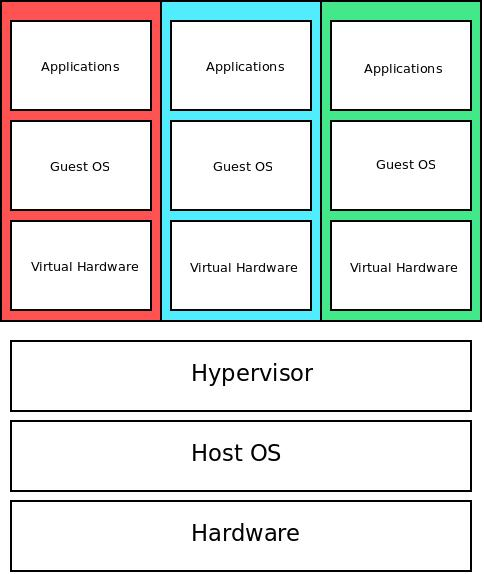
\includegraphics[width=10cm,height=10cm, keepaspectratio]{fullvirt.jpeg}%
  \caption{Full virtualisation architecture}
  \label{fig:full}
\end{figure}

The main advantage of full virtualisation is that it is easy to deploy and should not pose problems to an average user but the virtualisation overhead results in significantly reduced performance when compared to running directly on hardware. Popular examples of full virtualisation applications are Oracle's \textit{VirtualBox}\cite{VirtualBox} and \textit{VMware Workstation}\cite{WorkStation}. 

\subsubsection{Container-based virtualisation}

Instead of virtualising the underlying hardware, container-based virtualisation also known as OS-Layer virtualisation \cite{taxonomy} focuses on user space and allows running multiple operating systems in parallel as applications using the same kernel as the host operating system. A prime example of a popular container-based virtualisation platform is \textit{Docker} \cite{docker} which leverages on native Linux kernel features to virtualise and isolate OS instances. Figure ~\ref{fig:container} shows a container-based virtualisation architecture in which containerised environments are running operating systems on host OS's kernel. 

\begin{figure}[ht!]
\centering
  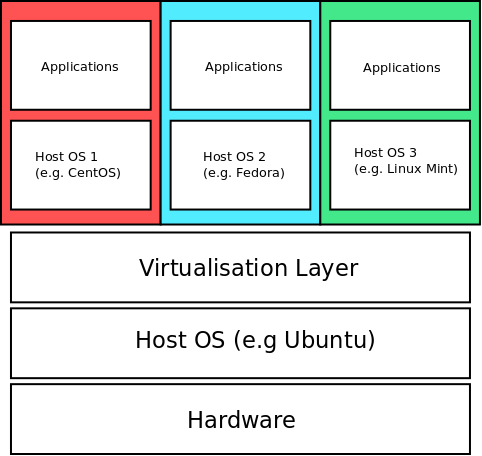
\includegraphics[width=10cm,height=10cm, keepaspectratio]{containers.png}%
  \caption{Container-based architecture}
  \label{fig:container}
\end{figure}

Container-based virtualisation does not need to emulate the hardware as containers communicate directly with the host kernel \cite{eder2016hypervisor} and are thus very fast to start. They also do not require all of the components a fully virtualised environment would need to run and therefore their resource fingerprint is minimal when compared to hypervisor-based virtualisation techniques. \linebreak
The obvious drawback of the technique is that the kernel of the virtualised OS has to be the same as that of Host OS e.g. In a situation depicted in figure ~\ref{fig:container} operating systems based on  Linux kernel could be ran on Ubuntu Host OS but OSs like Windows or OSX could not. On certain virtualisation platforms resource-intensive containers can also affect other containers detrimentally as the shared host OS's kernel is forced to spend its execution time on handling the instructions from the stressed container \cite{Xaviercontainer}.

\subsubsection{Hardware-Layer virtualisation}

\subsubsection{Paravirtualisation}



